\section{Model Explainability (Tiny-XAI)}
\label{sec:explainability}

A persistent barrier hindering the real-world adoption of machine learning in mission-critical agronomy is the ``black-box'' nature of complex classifiers. When an automated controller actuates an irrigation valve, agronomists require verifiable, physically grounded justification to ensure that the decision reflects authentic crop physiology rather than sensor calibration drift or transient electromagnetic noise. To provide this transparency without inflating edge compute budgets, we implement \textbf{Tiny-XAI} via TreeSHAP (SHapley Additive exPlanations)~\cite{lundberg2017unified}.

\begin{figure*}[!t]
\centering
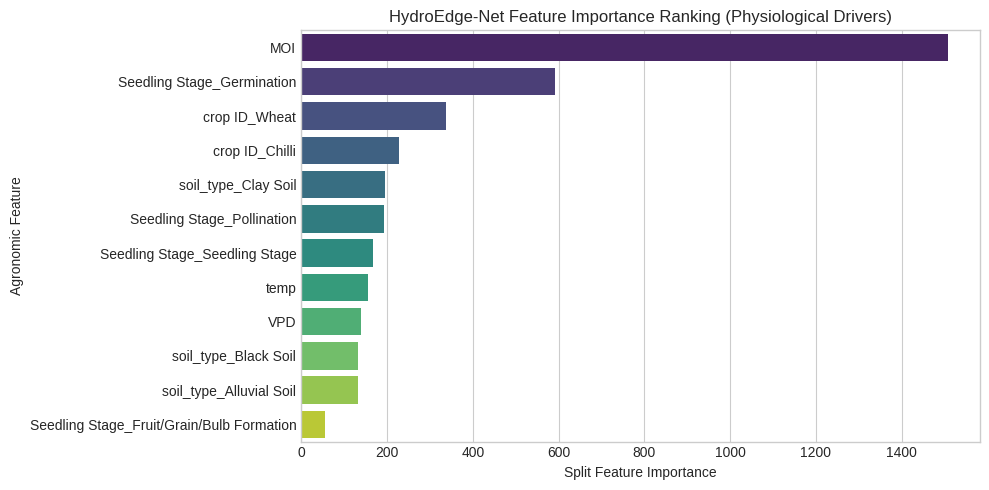
\includegraphics[width=0.92\textwidth]{figures/tinyxai_feature_importance.png}
\caption{Global and local feature importance ranking derived via Tiny-XAI (TreeSHAP) on the test split: (a) Mean absolute SHAP values across all features; (b) Beeswarm plot illustrating feature value impact on model output log-odds for water deficit stress.}
\label{fig:tiny_xai}
\end{figure*}

\subsection{TreeSHAP Attribution Formulation}

For a decision tree ensemble $f(\mathbf{x})$, TreeSHAP calculates the exact marginal contribution $\phi_j$ of each feature $j$ to the prediction $f(\mathbf{x})$ relative to the base expected value $\mathbb{E}[f(\mathbf{x})]$:
\begin{equation}
f(\mathbf{x}) = \phi_0 + \sum_{j=1}^{M} \phi_j(\mathbf{x})
\label{eq:shap_sum}
\end{equation}
where $\phi_0 = \mathbb{E}[f(\mathbf{x})]$, and the Shapley value $\phi_j$ satisfies local accuracy, missingness, and consistency axioms~\cite{lundberg2017unified}:
\begin{equation}
\phi_j(\mathbf{x}) = \sum_{S \subseteq F \setminus \{j\}} \frac{|S|!(|F| - |S| - 1)!}{|F|!} \left[ f_x(S \cup \{j\}) - f_x(S) \right]
\label{eq:shap_exact}
\end{equation}
Because HydroEdge-Net enforces strict depth clipping ($d \le 5$), the worst-case time complexity of TreeSHAP per sample scales as $O(N_{\text{trees}} \cdot L \cdot d^2)$, where $L \le 31$ is the maximum number of leaves, enabling rapid post-hoc attribution generation and deterministic computational tractability.

\subsection{Dominant Physiological Drivers and Agronomic Validation}

The global feature importance ranking and local impact beeswarm distribution generated by Tiny-XAI are presented in Fig.~\ref{fig:tiny_xai}. The empirical SHAP attributions reveal clear physiological alignments:
\begin{enumerate}
    \item \textbf{Soil Moisture Content ($\theta$ / MOI) as the Foundation:} Volumetric soil moisture emerges as the single most influential feature, accounting for a mean absolute SHAP value of $\sim 0.45$. In the beeswarm distribution (Fig.~\ref{fig:tiny_xai}b), low values of $\theta$ (blue points) exert massive positive SHAP impact pushing the log-odds strongly toward Class 1 (water deficit stress), whereas high $\theta$ values firmly anchor the prediction in Class 0 or Class 2.
    \item \textbf{High Marginal Utility of the $\Psi_{\text{TMS}}$ Coupling Index:} The proposed Thermal-Moisture Stress Coupling Index ranks as the second most dominant feature ($\text{mean } |\text{SHAP}| \approx 0.22$), surpassing raw temperature and raw humidity. This finding empirically confirms our core biophysical hypothesis: the predictive model relies heavily on the non-linear interaction between atmospheric vapor pull ($\text{VPD}$) and root-zone water depletion ($\text{SMD}/\theta_{\text{FC}}$). During periods where both atmospheric evaporative demand and soil moisture depletion are elevated, $\Psi_{\text{TMS}}$ spikes, driving immediate stress classification even before soil moisture reaches catastrophic wilting levels.
    \item \textbf{Atmospheric Evaporative Drivers (VPD and $T$):} Vapor Pressure Deficit and ambient air temperature provide the next tier of attribution. Elevated VPD values systematically increase stress probability, reflecting increased transpirational potential that accelerates soil water extraction.
    \item \textbf{Soil Texture and Phenological Stage Vulnerability:} Categorical encodings for soil type and phenological growth stage contribute meaningful marginal adjustments. In particular, early developmental stages (Seedling and Early Vegetative) exhibit higher baseline SHAP contributions toward stress sensitivity. Agronomically, young seedlings possess shallow, unestablished root architectures ($<15$~cm depth) with minimal volumetric soil reservoir access; consequently, they experience rapid desiccation under modest evaporative demand. In contrast, mature crops with deep taproots tolerate identical surface depletion without incurring water stress.
\end{enumerate}

By exposing these attributions, HydroEdge-Net guarantees that irrigation valve triggers are fully auditable, establishing trust for autonomous agricultural deployments.
